\documentclass[12pt]{article}

\usepackage{amssymb,amsmath,amsthm}
\usepackage[top=1in, bottom=1in, left=1.25in, right=1.25in]{geometry}
\usepackage{fancyhdr}
\usepackage{enumerate}
\usepackage[bw,framed,numbered]{mcode}
\usepackage{graphicx}

% Comment the following line to use TeX's default font of Computer Modern.
\usepackage{times,txfonts}

\newtheoremstyle{homework}% name of the style to be used
  {18pt}% measure of space to leave above the theorem. E.g.: 3pt
  {12pt}% measure of space to leave below the theorem. E.g.: 3pt
  {}% name of font to use in the body of the theorem
  {}% measure of space to indent
  {\bfseries}% name of head font
  {:}% punctuation between head and body
  {2ex}% space after theorem head; " " = normal interword space
  {}% Manually specify head
\theoremstyle{homework} 

% Set up an Exercise environment and a Solution label.
\newtheorem*{exercisecore}{Exercise \@currentlabel}
\newenvironment{exercise}[1]
{\def\@currentlabel{#1}\exercisecore}
{\endexercisecore}

\newcommand{\localhead}[1]{\par\smallskip\noindent\textbf{#1}\nobreak\\}%
\newcommand\solution{\localhead{Solution:}}

%%%%%%%%%%%%%%%%%%%%%%%%%%%%%%%%%%%%%%%%%%%%%%%%%%%%%%%%%%%%%%%%%%%%%%%%
%
% Stuff for getting the name/document date/title across the header
\makeatletter
\RequirePackage{fancyhdr}
\pagestyle{fancy}
\fancyfoot[C]{\ifnum \value{page} > 1\relax\thepage\fi}
\fancyhead[L]{\ifx\@doclabel\@empty\else\@doclabel\fi}
\fancyhead[C]{\ifx\@docdate\@empty\else\@docdate\fi}
\fancyhead[R]{\ifx\@docauthor\@empty\else\@docauthor\fi}
\headheight 15pt

\def\doclabel#1{\gdef\@doclabel{#1}}
\doclabel{Use {\tt\textbackslash doclabel\{MY LABEL\}}.}
\def\docdate#1{\gdef\@docdate{#1}}
\docdate{Use {\tt\textbackslash docdate\{MY DATE\}}.}
\def\docauthor#1{\gdef\@docauthor{#1}}
\docauthor{Use {\tt\textbackslash docauthor\{MY NAME\}}.}
\makeatother

% Shortcuts for blackboard bold number sets (reals, integers, etc.)
\newcommand{\Reals}{\ensuremath{\mathbb R}}
\newcommand{\Nats}{\ensuremath{\mathbb N}}
\newcommand{\Ints}{\ensuremath{\mathbb Z}}
\newcommand{\Rats}{\ensuremath{\mathbb Q}}
\newcommand{\Cplx}{\ensuremath{\mathbb C}}
%% Some equivalents that some people may prefer.
\let\RR\Reals
\let\NN\Nats
\let\II\Ints
\let\CC\Cplx

%%%%%%%%%%%%%%%%%%%%%%%%%%%%%%%%%%%%%%%%%%%%%%%%%%%%%%%%%%%%%%%%%%%%%%%%%%%%%%%%%%%%%%%
%%%%%%%%%%%%%%%%%%%%%%%%%%%%%%%%%%%%%%%%%%%%%%%%%%%%%%%%%%%%%%%%%%%%%%%%%%%%%%%%%%%%%%%
% 
% The main document start here.

% The following commands set up the material that appears in the header.

%%%%%%%%%%%%%%%%%%%%%%%%%%%%%%%%%%%%%%%%%%%%%%%%%%%%%%%%%%%%%%%%%%%%%%%%%%%%%%%%%%%%%%%
%%%%%%%%%%%%%%%%%%%%%%%%%%%%%%%%%%%%%%%%%%%%%%%%%%%%%%%%%%%%%%%%%%%%%%%%%%%%%%%%%%%%%%%
% 
% The main document start here.

% The following commands set up the material that appears in the header.
\doclabel{Math 310: Homework 4}
\docauthor{Parker Whaley}
\docdate{August 24, 2016}

\newcommand{\vv}{\mathbf{v}}
\begin{document}
\begin{exercise}

Chapter 4: 2 (c)
\end{exercise}
Here is my secant method:
\lstinputlisting{../octave/secant.m}
The driver code:
\lstinputlisting{../octave/secdrvr.m}
The output:
\lstinputlisting{../octave/4_7_2_a.txt}
Note that were I have a predicted a error in y and a actual error in y the two values are close (within a order of magnitude).  This is a good indication that the model used to predict errors is valid and so we can use this model to predict that to get the y error under $10^{-16}$ will take two more steps.

\begin{exercise}

Chapter 4: 3 (Just the last sentence of the problem)
\end{exercise}
Newton's method in this problem iterates as $\rho (x)=2x-x^2R$.  Solving for stability we get $\rho (x)=x$ or $x=2x-x^2R$, $0=x(1-xR)$, $x=0,1/R$.  This method will converge in a interval around $1/R$ where $|\rho'(x)|<1$, $|2-2xR|<1$, $-1<2-2xR<1$, $-3<-2xR<-1$, $\frac{3}{2}1/R>x>\frac{1}{2}1/R$, note that the fixed point $1/R$ is in this range.  So in the particular case where $1/R=1/3$ we get convergence where $\frac{1}{6}<x<\frac{1}{2}$.

\begin{exercise}

Chapter 4: 5
\end{exercise}
Nowhere does it say "solve by hand"!
\lstinputlisting{../octave/4_7_5.txt}

\newpage
\begin{exercise}

Chapter 4: 8
\end{exercise}
If we were attempting to find a root with secant method we would be using:
$$x_{k+1}=x_k-\frac{f(x_k)}{\frac{f(x_k)-f(x_{k-1})}{x_k-x_{k-1}}}$$
so:
$$x_{2}=x_1-\frac{f(x_1)}{\frac{f(x_1)-f(x_{0})}{x_1-x_{0}}}$$
$$-2=-1-\frac{4}{\frac{4-f(x_0)}{-1-2}}$$
$$-2=-1+\frac{3*4}{4-f(x_0)}$$
$$-1=\frac{12}{4-f(x_0)}$$
$$-12=4-f(x_0)$$
$$f(x_0)=16$$

\begin{exercise}

Chapter 4: 12
\end{exercise}
\begin{enumerate}[(a)]
\item
Fixed points are where $\rho(x)=x$ so $x^2+4=5x$, $x^2-5x+4=0$, $(x-1)(x-4)=0$, $x=1,4$.
\item
Basically is it true that $(\forall\xi\in [0,2]), |\rho'(\xi)|<1$.  Well $|\rho'(\xi)|=|\frac{2}{5}\xi|=\frac{2}{5}\xi$ and $0 \leq \frac{2}{5}\xi \leq \frac{4}{5}$.  Thus it is clearly true that $|\rho'(\xi)|<1$ and so these iteration will converge to $x=1$, $\forall x_0\in [0,2]$.
\end{enumerate}
\begin{exercise}

Chapter 4: 13
\end{exercise}
Consider the equation $\rho(y)=a+\epsilon \sin(y)$.  Note that the fixed points occur where $y=a+\epsilon sin(y)$, $y-\epsilon \sin(y)=a$.  Assume there are two distinct fixed points $x\neq y$ and $\rho(x)=x$, $\rho(y)=y$.  Note that $|x-y|=|\rho(x)-\rho(y)|=|\epsilon(\sin(x)-\sin(y)|$.  So $\frac{|x-y|}{\epsilon}=|\sin(x)-\sin(y)|$ if we note that $|x-y|\neq 0$ and $\frac{1}{\epsilon}>1$ we can see $|x-y|>\frac{|x-y|}{\epsilon}$ thus $|x-y|>|\sin(x)-\sin(y)|$.\\\\
Lets define $w=x-y$.  Note that $\sin(x)=\sin(y+w)$.  Doing a Taylor expansion about $w=0$ we get $\sin(x)=\sin(y+w)=\sin(y)+\cos(y+\xi)\xi$ where $\xi$ is between $w$ and 0, even though we don't know the sign of $w$ we can still say $|\xi|\leq |w|$.  Now note that $|\sin(x)-\sin(y)|=|\sin(y)+\cos(y+\xi)\xi-\sin(y)|=|\cos(y+\xi)\xi|\leq |\xi|\leq |w|=|x-y|$.  Thus $|\sin(x)-\sin(y)|\leq |x-y|$\\\\
Combining these two parts we get $|x-y|>|\sin(x)-\sin(y)|\geq |x-y|$ in other words $|x-y|>|x-y|$, a contradiction.  We conclude the negation of our supposition, namely that there does not exist two fixed points to our $\rho(y)$ and thus if there is a solution it is unique.\\
Noting that $a+\epsilon \sin(0)-0\geq 0$ and $a+\epsilon \sin(2 \pi)-2\pi=a-2\pi<0$ we conclude that there is a solution in $[0,2\pi)$.  Thus there is a unique fixed point.
\newpage
\begin{exercise}

Chapter 4: 14
\end{exercise}
We are iterating $\rho(y)=\cos(y)$.\\\\
Fixed points must occur where $y=\cos(y)$.  Note that fixed points must occur in $y\in [-1,1]$ since $|y|=|\cos(y)|\leq 1$.  Fixed points are also solutions to $\cos(y)-y=0$, noting that $-\sin(y)-1<0$, $y\in[-1,1]$ we can say $\cos(y)-y$ is monotonically decreasing $y\in[-1,1]$ and thus there is at most one zero, and so if there is a fixed point it is unique.  Noting that $\cos(0)-0=1>0$ and $\cos(1)-1\approx -.5<0$, we can say that there is a fixed point in $y\in[0,1]$.  Thus there is a unique fixed point and it is between 0 and 1.\\\\
What happens as we iterate on $y$, $y\in [-1,1]$?  In this range $|\rho'(y)|=|sin(y)|<1$, thus in this range of $y$ we converge to the fixed point.  Note that if we start with a $y$ outside of this range we are guaranteed by the range of $\cos$ that $\rho(y)\in[-1,1]$, thus all values of $y$ converge to the fixed point somewhere between 0 and 1.  Experimentally this value is about $0.73909$.
\begin{exercise}

Chapter 4: 15
\end{exercise}
We are asked to discuss how $\rho(x)=\frac{1}{2}(-x^2+x+2)$ behaves with $x_0=.5$, given that it has a fixed point at $x=1$.  Note that $\rho'(x)=-x+.5$ and so in the interval $x\in(.5,1.5)$ $|\rho(x)|<1$, $\rho(x)$ converges to $1$.  Noting that $\rho(.5)\approx 1.1\in(.5,1.5)$ we can say that $\rho(x)$ converges to $1$ if we start with $x_0=.5$.\\\\
Assume that the convergence takes the form $\frac{|err_{k+1}|}{|err_k|^\alpha}\rightarrow C$ as $x_k\rightarrow 1$.  Note that $$\lim_{err\rightarrow 0}\frac{|err_{k+1}|}{|err_k|^\alpha}=\lim_{x\rightarrow 1}\frac{|\rho(x)-1|}{|x-1|^\alpha}=C$$
$$\lim_{x\rightarrow 1}\frac{|\rho(x)-1|}{|x-1|^\alpha}=
\lim_{x\rightarrow 1}\frac{|-x^2/2+x/2+1-1|}{|x-1|^\alpha}=
\lim_{x\rightarrow 1}\frac{|-x/2||x-1|}{|x-1|^\alpha}$$
assuming $\alpha=1$
$$=\lim_{x\rightarrow 1}|-x/2|=1/2$$
So we conclude $\frac{|err_{k+1}|}{|err_k|}\rightarrow 1/2$ as $x_k\rightarrow 1$, thus this converges linearly.\\\\
I wrote a script that illustrates this convergence by plotting the error and the predicted error using the above model.\\
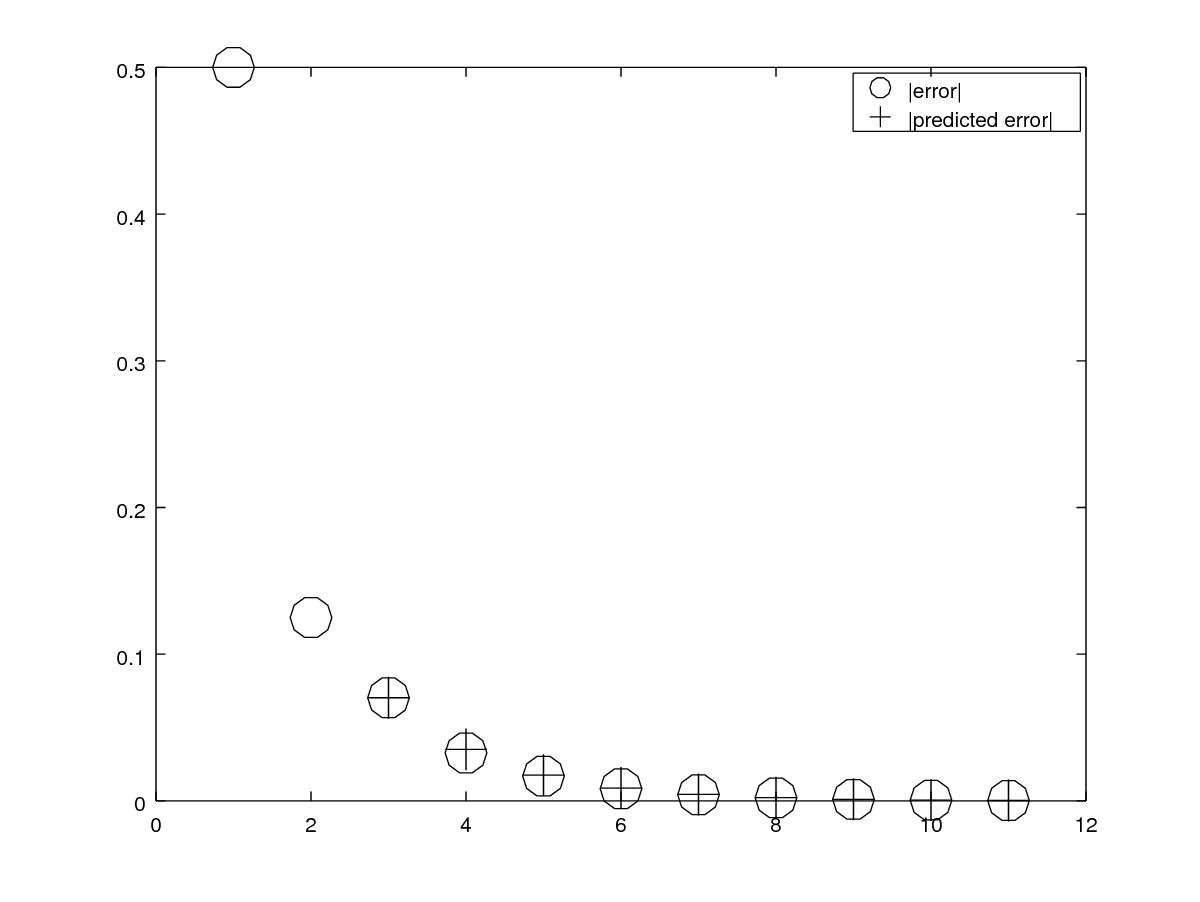
\includegraphics[scale=.5]{../octave/f1.jpg}\\
The similarity is even more apparent in a log plot.\\
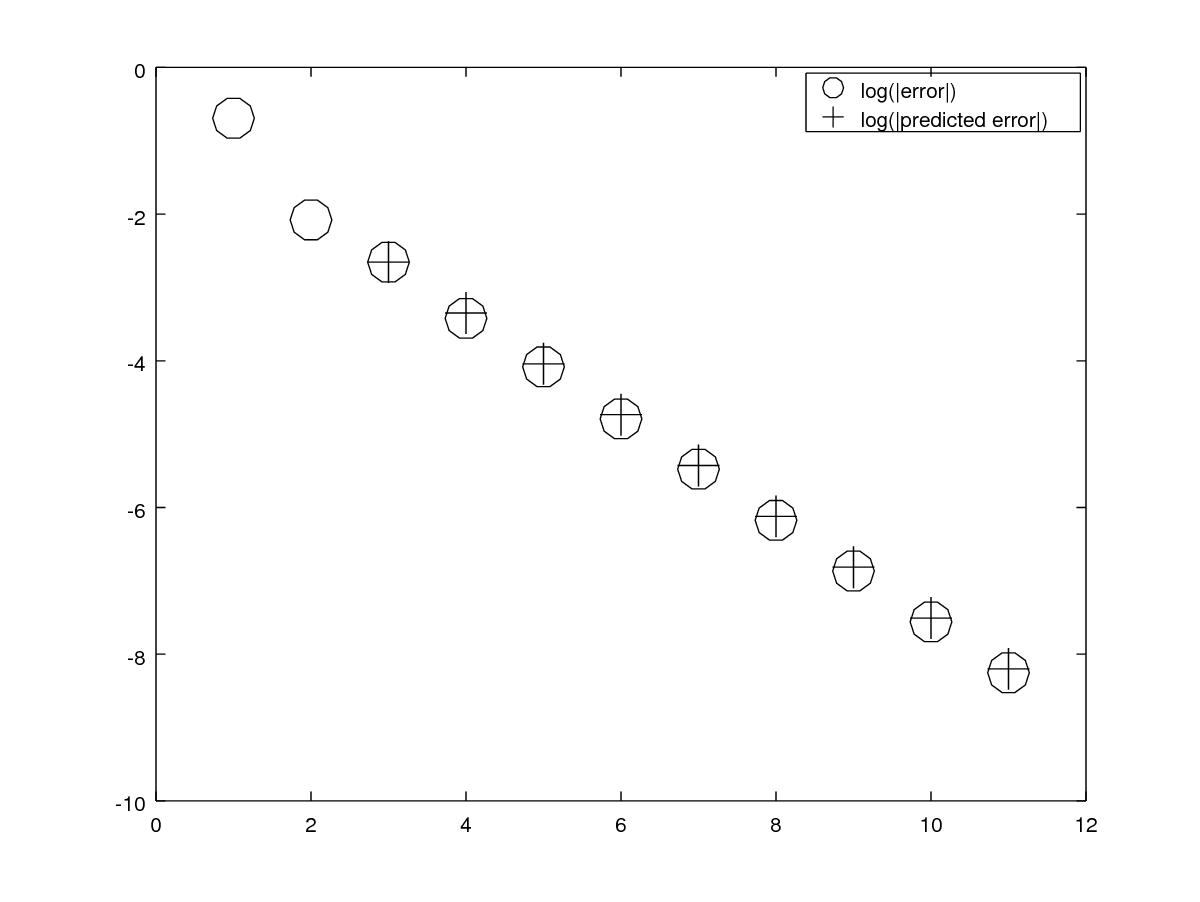
\includegraphics[scale=.5]{../octave/f2.jpg}\\
These graphs clearly show that the predicted end behavior is correct and that the absolute value of the error is halved with each iteration.\\
\newpage
Driver code:
\lstinputlisting{../octave/q4_15.m}
Output:
\lstinputlisting{../octave/d_q15.txt}
\end{document}